\chapter{Coarse-grained Cross Modal Retrieval}
\label{cha:scan}
In Chapter \ref{cha:relatedworks}, we discussed several models proposed to solve the image-text alignment task. However, they all have drawbacks in terms of different aspects. In this chapter we explain the \textbf{S}tacked \textbf{C}ross \textbf{A}ttentio\textbf{n} Model (SCAN) \cite{scan} and applied it on performing coarse-grained cross-modal retrieval task. Followed by discussing how it surpasses other models and why we choose to investigate it to solve the problem later in the task of fine-grained cross-modal retrieval for artworks.

The structure of this chapter is as follows. Section 3.1 gives an introduction and motivation of SCAN. Section 3.2 explains the structure and methodologies used in SCAN, also how all its components iterates with each other. Section 3.3 briefly discusses the strengths of the adopted model for coarse-grained cross-modal retrieval. Section 3.4 illustrates the preliminary experimental results on our artwork datasets and the achievement of SCAN. Section 3.5 summarises this section.

\section{Motivation}

There are several models proposed recently to solve the problem of cross-modal retrieval, and many have achieved excellent accomplishments. However, Lee, et al. \cite{scan} mentioned some current existing drawbacks of mainstream image-text alignment models, such as:

\begin{itemize}
    \item Attention mechanism is not considered at all, and the entire image and sentence pair are aggregated together, e.g. VSE++ \cite{vse}.
    \item A bit more refined: calculate the similarity between each region-word, take maximum and add them together as the similarity of the entire pair, e.g. Deep-VS \cite{neuraltalk2}.
    \item With attention used, but a predetermined step-process is used to capture limited semantic alignment, and because the entire feature is sent in, it lacks interpretability, e.g. Dual Attention Networks (DANs) \cite{dan}.
\end{itemize}

Stacked Cross Attention (SCAN) is proposed in a paper published on ECCV by Lee, et al. \cite{scan} in 2018. The paper aimed to combine the above aspects (attention mechanism and using pairs), first extracting the features of the image and sentence, then using attention for each region and word, and finally calculating similarity so that attention is used for finer-grained alignment.

Also, the paper used some of the currently available optimisation methods, such as the use of hard-negative, triplet ranking loss, etc.

We explain the structure of SCAN model in the next sections.

\section{Image Feature Extraction}
Before we perform any cross-modal retrieval and alignment between image and text, we need to have firstly extract features from images. There are many models we have discussed before in Section \ref{cha:relatedworks}, here we used one of the mentioned models called Faster R-CNN. 

Anderson, et al. \cite{bottomup} proposes a top-down and bottom-up attention model method, which is applied to the related issues of visual scene understanding and prominent question answering system. This is based on the bottom-up attention model (usually Faster R-CNN) is used to extract the region of interest in the image. 

Although this work \cite{bottomup} does not mention the Encoder-Decoder framework, which is the most widely used in the current research, the task of the bottom-up attention model is to obtain the image interest area. Extracting image features is similar to feature encoding the image to achieve the encoding stage Task; and the top-down attention model is used to learn to adjust the feature weights, realise the ``timely attention'' of image content, and generate descriptions word by word, equivalent to the decoding stage.


\subsection{Why Adopt Faster R-CNN?}

\begin{figure}[h!]
\centering
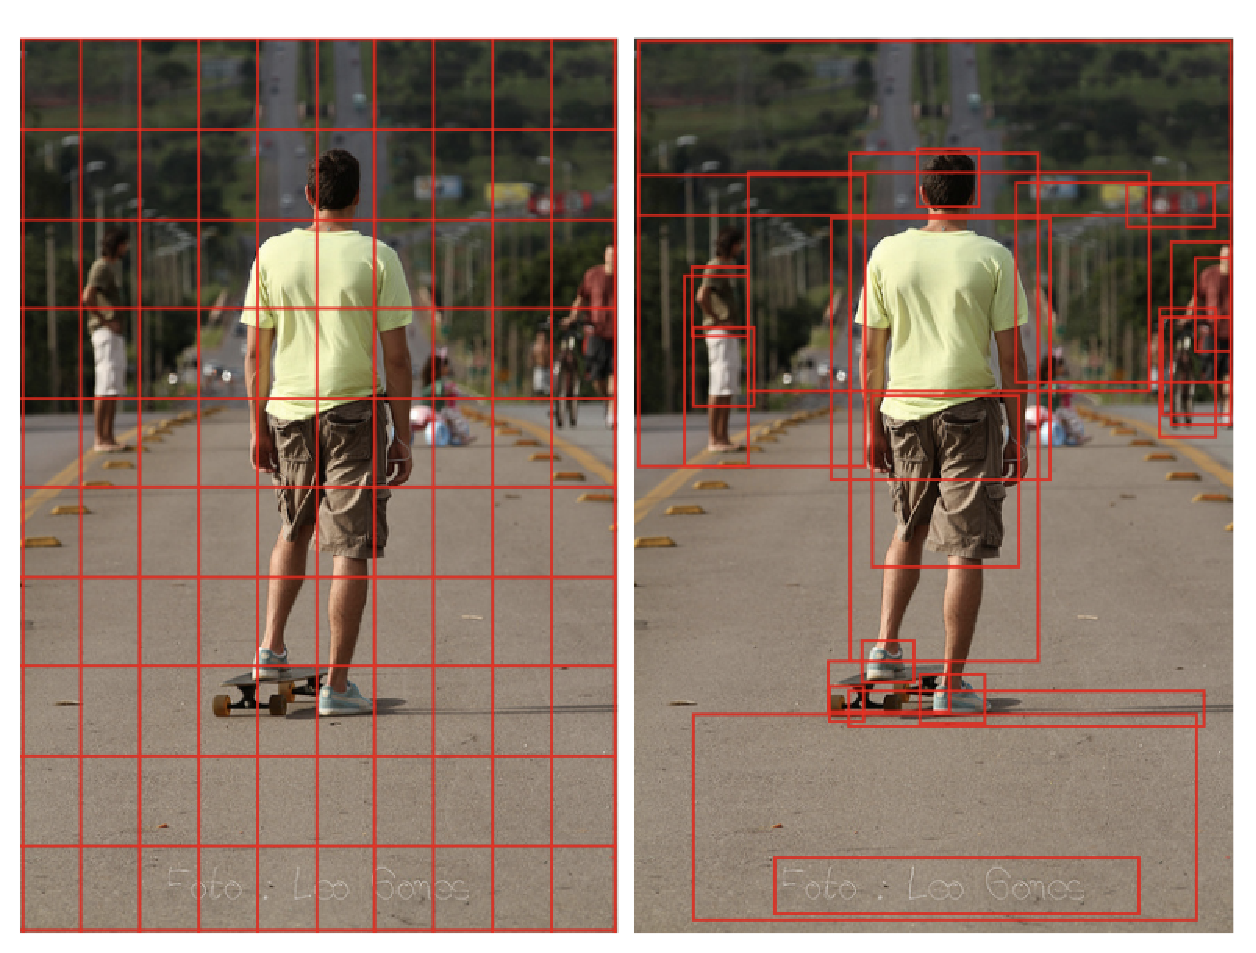
\includegraphics[width=.4\textwidth]{whyfasterrcnn.pdf}
\caption{Faster R-CNN with attention comparing to CNN \cite{bottomup}}
\label{fig:fasterrcnnbottomup}
\end{figure}

It can be seen from the Figure \ref{fig:fasterrcnnbottomup} that using CNN requires more features than R-CNN, and many features are often useless. The target detection method of R-CNN first obtains the interest area for the image, and then applies the target detector to each interest area, so that the image category can be accurately obtained; the CNN method requires the input of the entire image and is used for broad sample classification Of networks are often complex and computationally intensive. In addition, Faster R-CNN improves on previous generations of R-CNN methods and realises the ability to recognise all objects with only one input, which significantly improves processing efficiency.

\subsection{Bottom-Up Attention Model}

From Figure \ref{fig:bottomup} below, it can be seen that the difference from the prior works is that the set of thresholds allows overlapping of interest frames, which can more effectively understand the image content. In this paper, not only the object detector but also the attribute classifier is used for each region of interest, so that a binary description of the object \verb|(attribute, object)| can be obtained. This description is more suitable for practical applications.

\begin{figure}[h!]
\centering
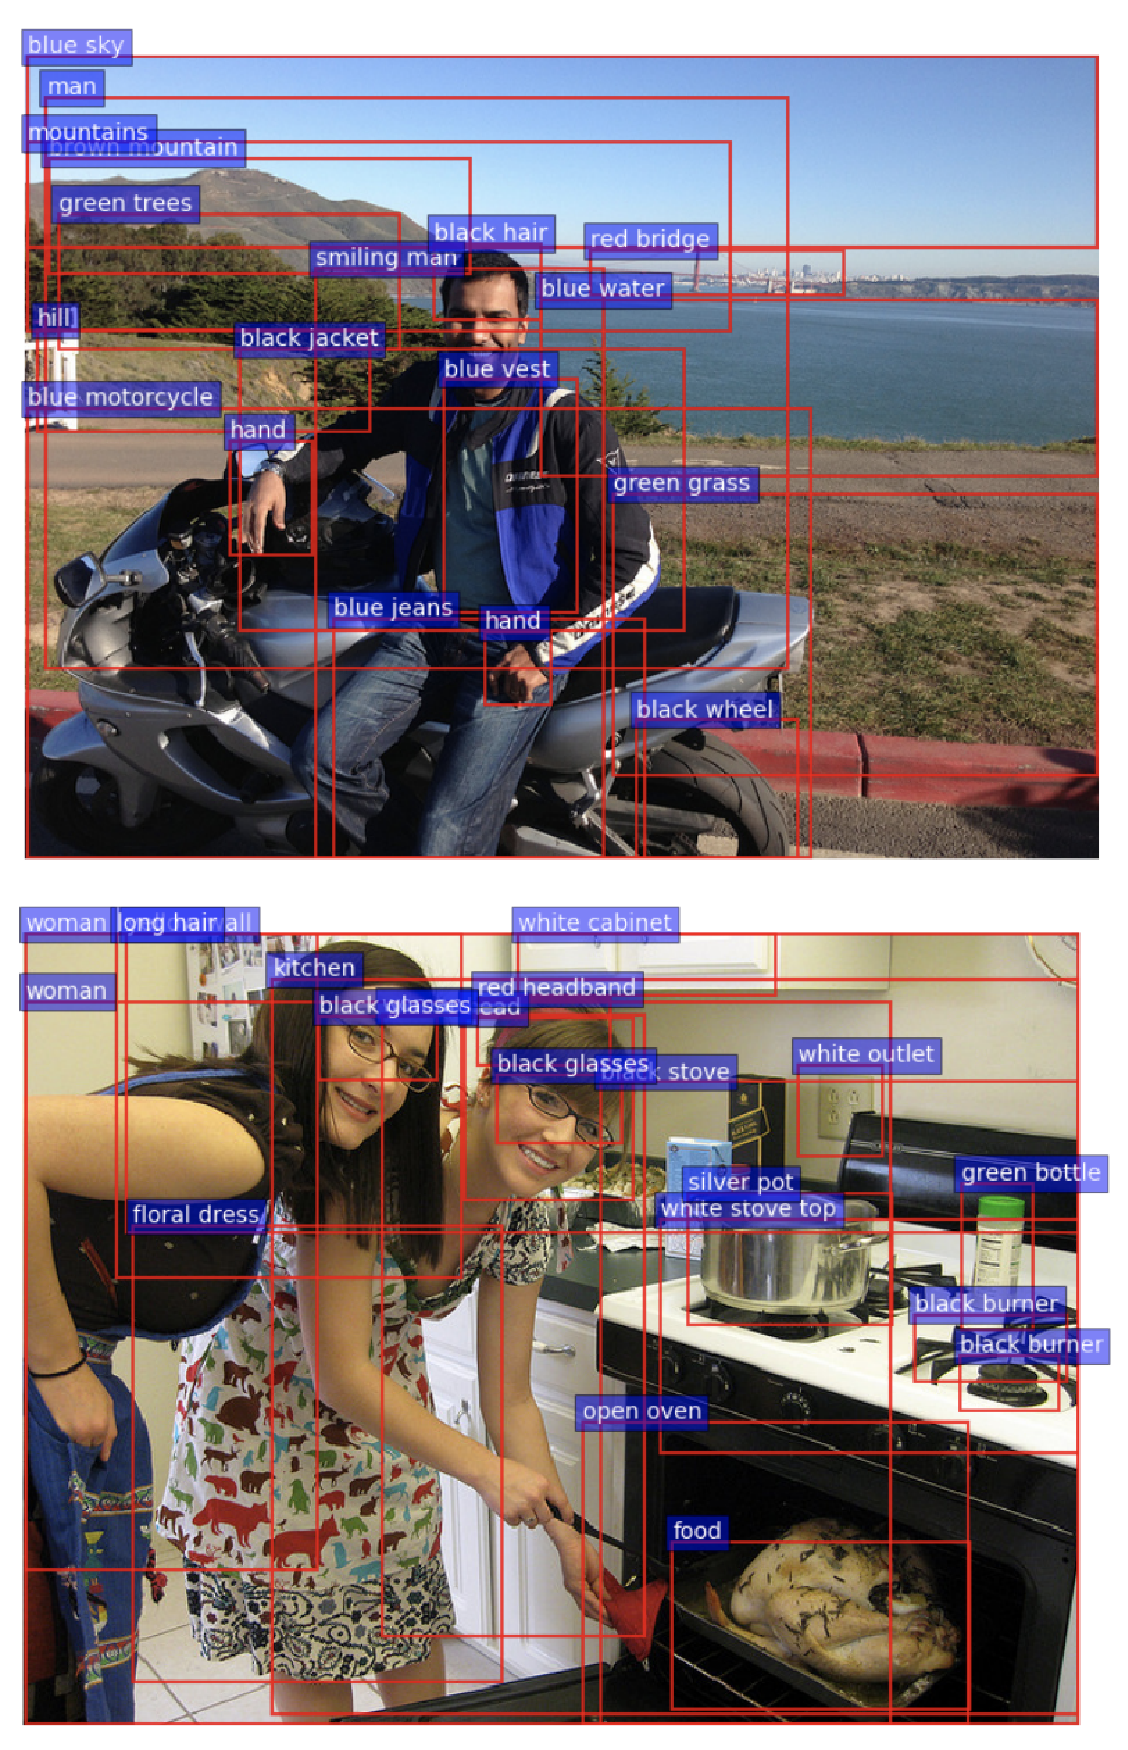
\includegraphics[width=.35\textwidth]{bottomup.pdf}
\caption{What bottom-up attention model captures? \cite{bottomup}}
\label{fig:bottomup}
\end{figure}

\section{SCAN Model}
In this section, we start discussing SCAN with a brief introduction on its structure, followed by in-depth explanations on each specific stages - what is happening behind and why?

\subsection{Brief Structure}
\begin{enumerate}
    \item Use bottom-up attention mechanism \cite{bottomup} to detect the image area and extract the features of the image area;
    \item Map the words in the sentence and their sentence context to feature vectors;
    \item Stacked Cross Attention is used to deduce the similarity of images and text by aligning image regions and word features;
    \item The loss function of SCAN focuses on the hardest negative image-text pairs in each batch (that is, the most unmatched image-text pairs).
\end{enumerate}

Next, we are going to explain each stage in detail.

\subsection{Image-Text Matching}

The process is shown below in Figure \ref{fig:scan1}.

\begin{figure}[h!]
\centering
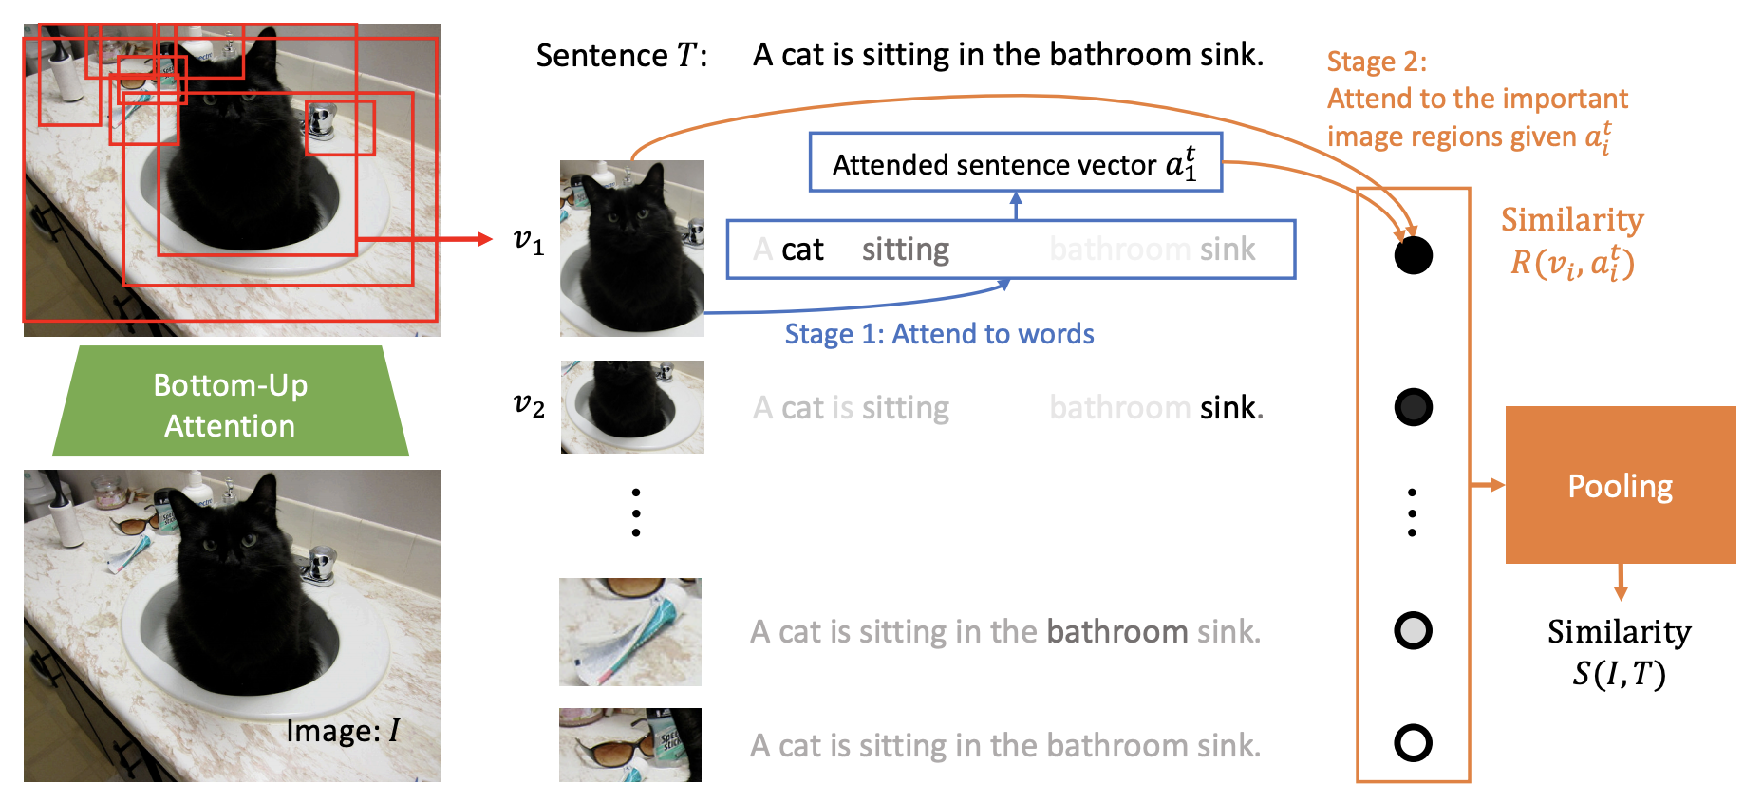
\includegraphics[width=1\textwidth]{scan1.pdf}
\caption{Image-Text Stacked Cross Attention \cite{scan}}
\label{fig:scan1}
\end{figure}

First, use bottom-up attention \cite{bottomup} to extract multiple proposals into features for the image, then map to the same dimensions as the sentence features, and use bi-direction GRU to extract features for the sentence.

Stage 1: calculate the attention representation $a_{i}^{t}$ of all words for each region $i$, and add them together to obtain the sentence representation $a_{i}^{t}$, the formula is as follows:

$$
a_{i}^{t}=\sum_{j=1}^{n} \alpha_{i j} e_{j}
$$

where

$$
\alpha_{i j}=\frac{\exp \left(\lambda_{1} \bar{s}_{i j}\right)}{\sum_{j=1}^{n} \exp \left(\lambda_{1} \bar{s}_{i j}\right)}
$$

Stage 2: calculate the cosine similarity of the $i$-th region and the obtained $a_{i}^{t}$.

$$
R\left(v_{i}, a_{i}^{t}\right)=\frac{v_{i}^{T} a_{i}^{t}}{\left\|v_{i}\right\|\left\|a_{i}^{t}\right\|}
$$

Finally, $i$ areas are superimposed together to get the similarity between image and text, using LogSumExp pooling (LSE), i.e.

$$
S_{L S E}(I, T)=\log \left(\sum_{i=1}^{k} \exp \left(\lambda_{2} R\left(v_{i}, a_{i}^{t}\right)\right)\right)^{\left(1 / \lambda_{2}\right)}
$$

Alternatively, we can
summarise $R\left(v_{i}, a_{i}^{t}\right)$ with average pooling (AVG), i.e.

$$
S_{A V G}(I, T)=\frac{\sum_{i=1}^{k} R\left(v_{i}, a_{i}^{t}\right)}{k}
$$

\subsection{Text-Image Matching}

\begin{figure}[h!]
\centering
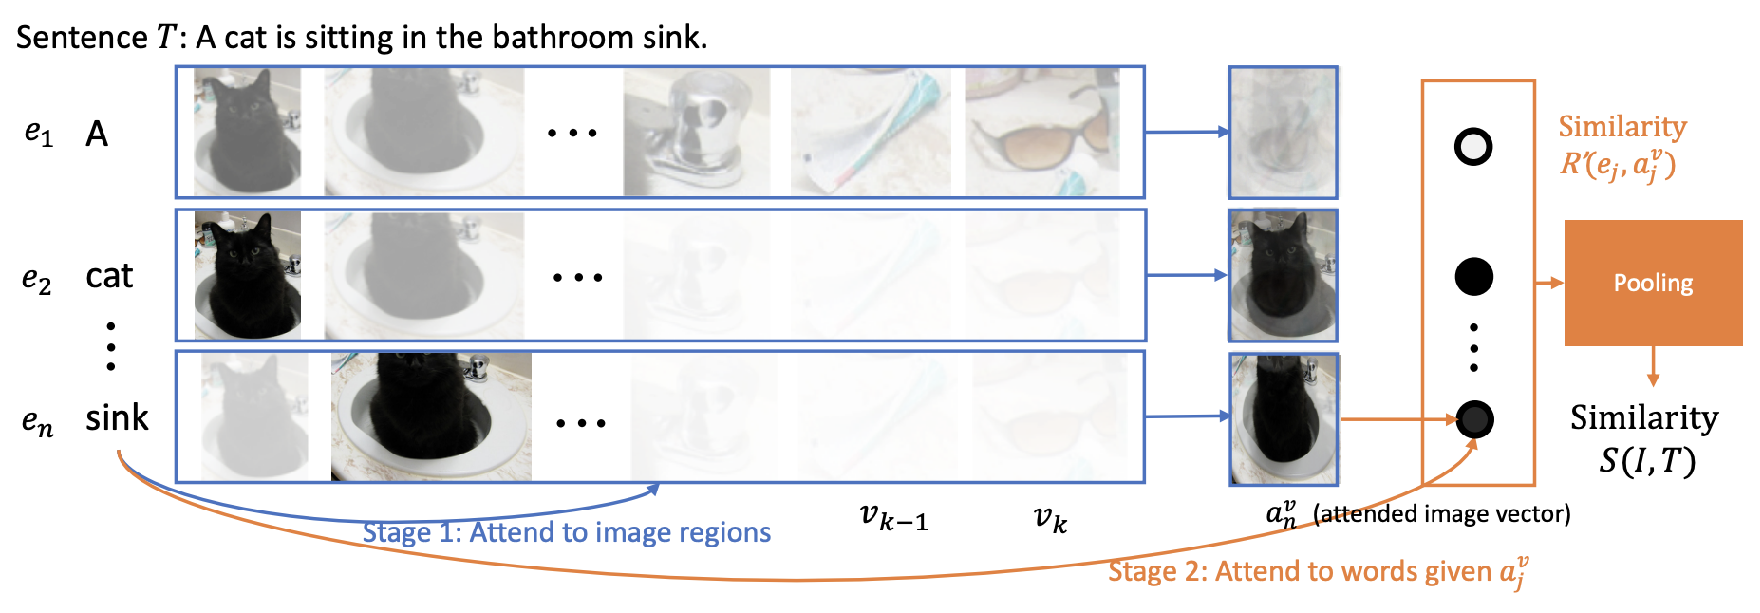
\includegraphics[width=1\textwidth]{scan2.pdf}
\caption{Text-Image Stacked Cross Attention \cite{scan}}
\label{fig:scan2}
\end{figure}

The overall steps correspond exactly to the above, except that each word is used to calculate the similarity with the attention of a picture, which is not repeated here. The process is illustrated in Figure \ref{fig:scan2}.

\subsection{Target Alignment}
Target alignment is essentially the setting of the loss function. In this case, SCAN employs a hinge-based triplet ranking loss with margin $\alpha$.

$$
l(I, T)=\sum_{\hat{T}}[\alpha-S(I, T)+S(I, \hat{T})]_{+}+\sum_{\hat{I}}[\alpha-S(I, T)+S(\hat{I}, T)]_{+}
$$

\begin{itemize}
    \item where $[x]_{+} \equiv \max (x, 0)$ and $S$ is similarity score function (e.g. $S_{L S E}$)
    \item The first sum is taken over all negative sentences $\hat{T}$ given an image $I$; the second sum considers all negative images $\hat{I}$ given a sentence $T$.
    \item If $I$ and $T$ are closer to one another in the joint embedding space than any negatives pairs, by the margin $\alpha$, the hinge loss is zero.
\end{itemize}

For computational efficiency, rather than summing over all the negative samples, it usually considers only the hard negatives in a mini-batch of stochastic gradient descent.

\begin{itemize}
    \item for a pair $(I, T)$, the formula is shown below. e.g. the hard negative of one image is the image that has the highest similarity with the text besides this original pair. (vice versa for text)
    \item Now the hardest negatives are given by $$\hat{I}_{h}=\operatorname{argmax}_{m \neq I} S(m, T)$$ and $$\hat{T}_{h}=\operatorname{argmax}_{d \neq T} S(I, d)$$
    \item The final loss is: 
    $$l_{h a r d}(I, T)=\left[\alpha-S(I, T)+S\left(I, \hat{T}_{h}\right)\right]_{+}+\left[\alpha-S(I, T)+S\left(\hat{I}_{h}, T\right)\right]_{+}$$
\end{itemize}

\subsection{Image and Text Feature Representation}

\subsubsection{Image}Bottom-up attention technique \cite{bottomup}, which is a method of target detection, is obtained based on faster-RCNN. Faster R-CNN first obtains the area of interest for the image, and then applies a target detector to each area of interest, so that the image features can be accurately obtained.

In this paper, the flow for image feature representation is: faster-RCNN, Residual NN (Resnet)101 $\Rightarrow$ 2,048 dimensional features $\Rightarrow$ fully-connected layer transform to $h$-dimensional $\Rightarrow$ get feature set $v$.

\subsubsection{Text}A RNN (recurrent neural networks) is used. In this paper, the flow for text feature representation is: word $\Rightarrow$ one-hot vector showing an index of the word in vocab $\Rightarrow$ embed to 300-dimensional vector $\Rightarrow$ bidirectional GRU map to $h$ dimensions word feature.

\section{Contribution}
Lee, et al. \cite{scan} uses the proposed \textbf{S}tacked \textbf{C}ross \textbf{A}ttentio\textbf{n} (SCAN) to find all potential alignments between the image area and the words, thereby calculating the similarity between the graphics and the text. Existing methods perform fixed-step attention inference so that only a limited semantic alignment can be found at a time, and SCAN can find all possible semantic alignments at the same time. Since the number of semantic alignments varies with different images and sentences, the corresponding relationship inferred by the Stacked Cross Attention method is more comprehensive, thereby making the image-text matching more interpretable.


\section{Preliminary Results}
Here we ran SCAN on two artwork datasets: one ancient Egyptian artworks and one Chinese artworks. For ancient Egyptian artworks dataset, it has 14,353 images in the training set, 1,793 images in the testing/validation set. The other Chinese artworks dataset, there are 6,086 images in the training set, 761 images in the testing/validation set.

For experiment settings, we tested on a Ubuntu machine with Intel Xeon Processor E5-1620 (10M Cache, 3.60 GHz) CPU and a GeForce GTX TITAN X GPU. The specific parameters settings are listed below:

\subsubsection{Settings for image representation}

\begin{itemize}
    \item We used faster R-CNN model and ResNet-101 model pre-trained by \textit{Anderson et al.} on \verb|Visual Genomes| dataset, performs detection of salient regions as bottom-up attention to extract features from images. 
    \item We captured 36 Region of Interests (ROIs) for each image after average pooling and extracted 2,048-dimensional features vector.
    \item We used L2 normalisation (Euclidean distance) into 1,024 joint embedding spaces (same for GRU), these will be used as image feature vectors.
\end{itemize}

\subsubsection{Settings for text representation}

\begin{itemize}
    \item We obtained 300 dimensional word embedding as input to GRU then use embedding matrix to map it into 1,024 joint embedding spaces.
\end{itemize}

\subsection{Results}

The following Table \ref{table:resultscan} illustrates the results of running SCAN model on our ancient Egyptian and Chinese art alignment datasets.

\begin{table}[h!]
\centering
\begin{tabular}{lllllll}
                       & \multicolumn{3}{c}{Sentence Retrieval} & \multicolumn{3}{c}{Image Retrieval} \\ \hline
method                 & R@1         & R@5         & R@10       & R@1        & R@5        & R@10      \\ \hline
\multicolumn{1}{r}{}   & \multicolumn{6}{c}{Ancient Egyptian art alignment dataset}                   \\ \hline
SCAN i-t AVG & 15.3        & 38.5        & 49.9       & 14.1       & 37.6       & 50.2      \\ \hline
\multicolumn{1}{r}{}   & \multicolumn{6}{c}{Ancient Chinese art alignment dataset}                    \\ \hline
SCAN i-t AVG & 3.3         & 20.4        & 36.1       & 8.0        & 22.9       & 33.8     
\end{tabular}
\caption{Result of SCAN on Artwork Datasets}
\label{table:resultscan}
\end{table}

The results are beyond satisfactory as shown; however, as in this stage, we only used the features obtained using bottom-up attention \cite{bottomup} to train and test, the result may be misleading. As bottom-up attention model was trained on natural images, which means the features we obtained for training and testing set may be irrelevant to those contained in artworks. Noted using entire artwork image and sentence caption to feed SCAN may also lose detailed information in artworks, which will be further discussed in Chapter \ref{cha:Method}.

\subsection{Examples}
Below we display a few examples from our coarse-grained cross modal retrieval model: one for each dataset under sentence retrieval and image retrieval.

\subsubsection{Sentence Retrieval}
Figure \ref{fig:scani2t} illustrates two examples which obtained textual attributes from image queries. There are several characteristics were successfully obtained from the left Egyptian anthropoid statue and the right Chinese vase including the shape and colour but not in a fragment level. That is, for example, our textual retrieval results captured ``dark brown mummy'', ``white porcelain vase'' and even a little bit detail: ``dark inscription on neck'', however, more details need to be furnished such as ``long thin beard'' and ``red flowers''. These cannot be accomplished well under the current settings we used which is coarse - based on image and sentence level.

\begin{figure}[h!]
\centering
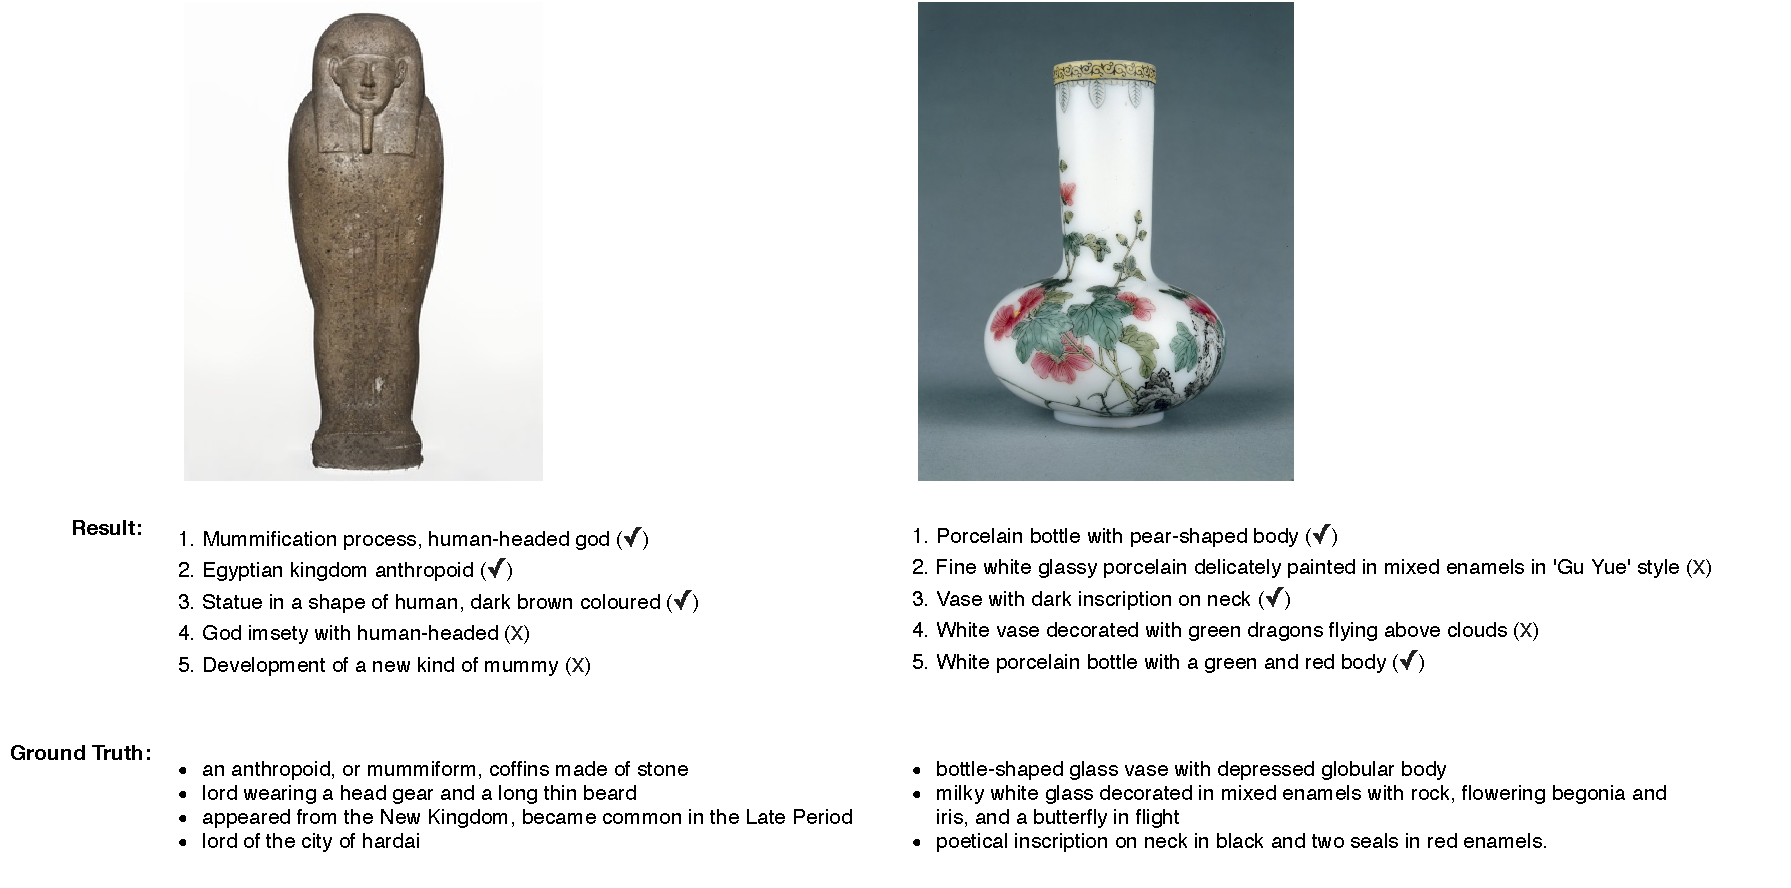
\includegraphics[width=1\textwidth]{scani2t.pdf}
\caption{Text Retrieval Example for Given Image Queries (coarse-grained)}
\label{fig:scani2t}
\end{figure}

\subsubsection{Image Retrieval}
Similar results appeared in image retrieval examples shown as Figure \ref{fig:scant2i}. The model was able to pick out major shapes and overall structure but detailed information cannot be well aligned between image and text thus cause inaccurate retrieval on a more fine-grained level.

\begin{figure}[h!]
\centering
\includegraphics[width=1\textwidth]{scant2i.pdf}
\caption{Image Retrieval Example for Given Text Queries (coarse-grained)}
\label{fig:scant2i}
\end{figure}


\section{Conclusion}
Automated image-text mutual annotation would benefit transforming traditional library artwork collection to digital. In this section, we employed a well-known cross modal retrieval model: Stacked Attention and evaluated our Egyptian and Chinese artwork datasets on it. Considering the unique representation of artworks, in the next chapter, we modify this current model to achieve the cross modal retrieval in a fine-grained level.


%%% Local Variables: 
%%% mode: latex
%%% TeX-master: "thesis"
%%% End: 
